\section{Sensors and Components}

\subsubsection*{Xsens Legacy}

\begin{itemize}
    \item It's a IMU thats has a magnetometer
\end{itemize}

\subsubsection*{Livox Mid-70}

\begin{itemize}
    \item Its a LiDAR
    \item Has a narrow FOV
\end{itemize}

\subsubsection*{Mynt Eye S1030}

\begin{itemize}
    \item RGB-D
    \item Wide FOV to complement the Livox narrow FOV
\end{itemize}

\subsubsection*{Intel Realsense D435i}

\begin{itemize}
    \item Near InfraRed, RGBD
\end{itemize}

\subsubsection*{Udoo Bolt v3}

\begin{itemize}
    \item Small factor computer 
    \item Arm CPU
    \item M.2 SSD to store the data
\end{itemize}

\subsubsection*{Turnigy battery}


\section{Eletronics}

\todo[inline]{Add eletronics flowchart here}

\section{Mechanical Structure}

The mechanical structure was divided in two diferent components, the sensor box, responsible for housing all cameras and sensors and by the backpack, reponsible for housing the computing, battery and eletronic components.

\begin{figure}[H]
    \centering
    \begin{subfigure}{0.45\textwidth}
        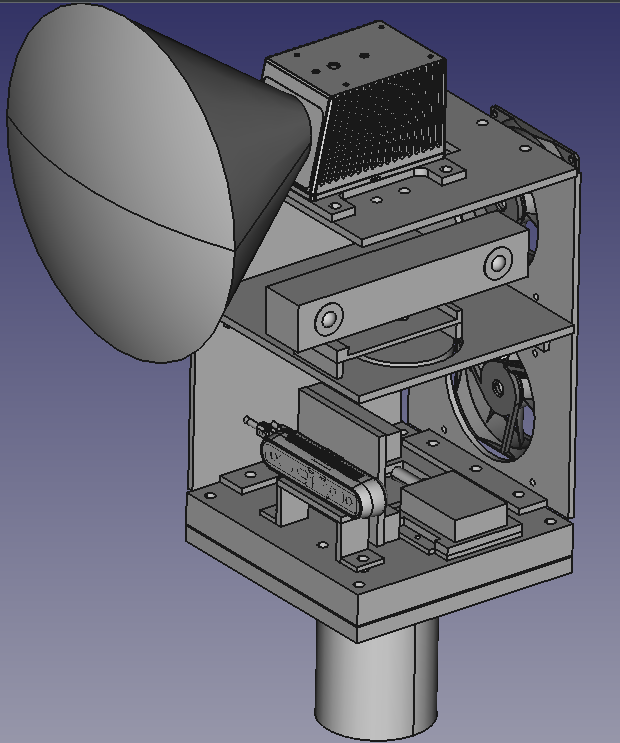
\includegraphics[width=0.9\linewidth]{images/sensor_box.png} 
        \caption{Sensor Box}
        \label{fig: sensor box}
    \end{subfigure}
    \begin{subfigure}{0.45\textwidth}
        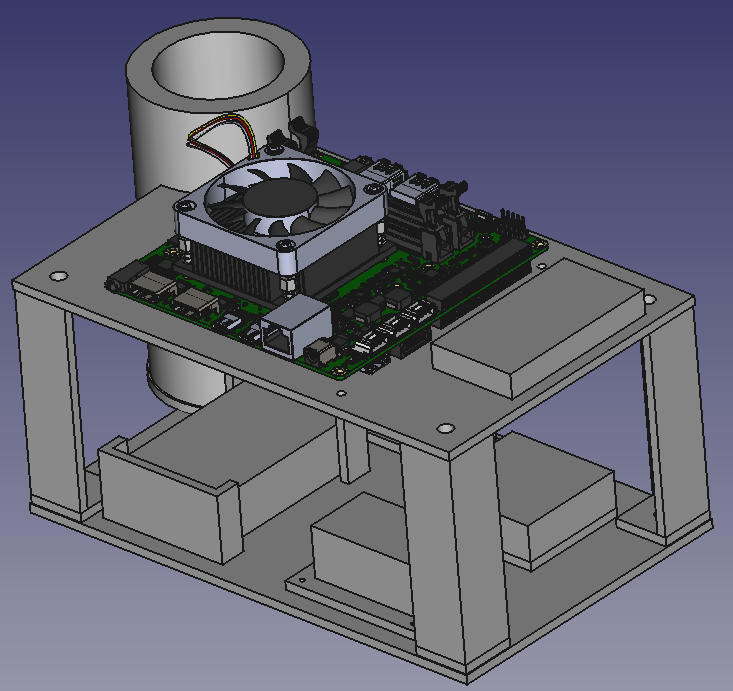
\includegraphics[width=0.9\linewidth]{images/backpack_skeleton.png}
        \caption{Backpack skeleton}
        \label{fig: backpack skeleton}
    \end{subfigure}
    \caption{CAD model of the structure}
    \label{fig: mechanical structure}
\end{figure}


In order to comply with the modularity requirement, the LiDAR component was put on top, since it is relatively common to have 360degrees LiDARs.







To assure the integraty of the apparatus, stress and frequency tests were performed to the sensor box component. The stress tests were perform in the open source software FreeCAD, and it used the Gmsh to create the mesh and the Calculicx the backend engine resposible to compute the dislocations.

\begin{figure}[H]
    \centering
    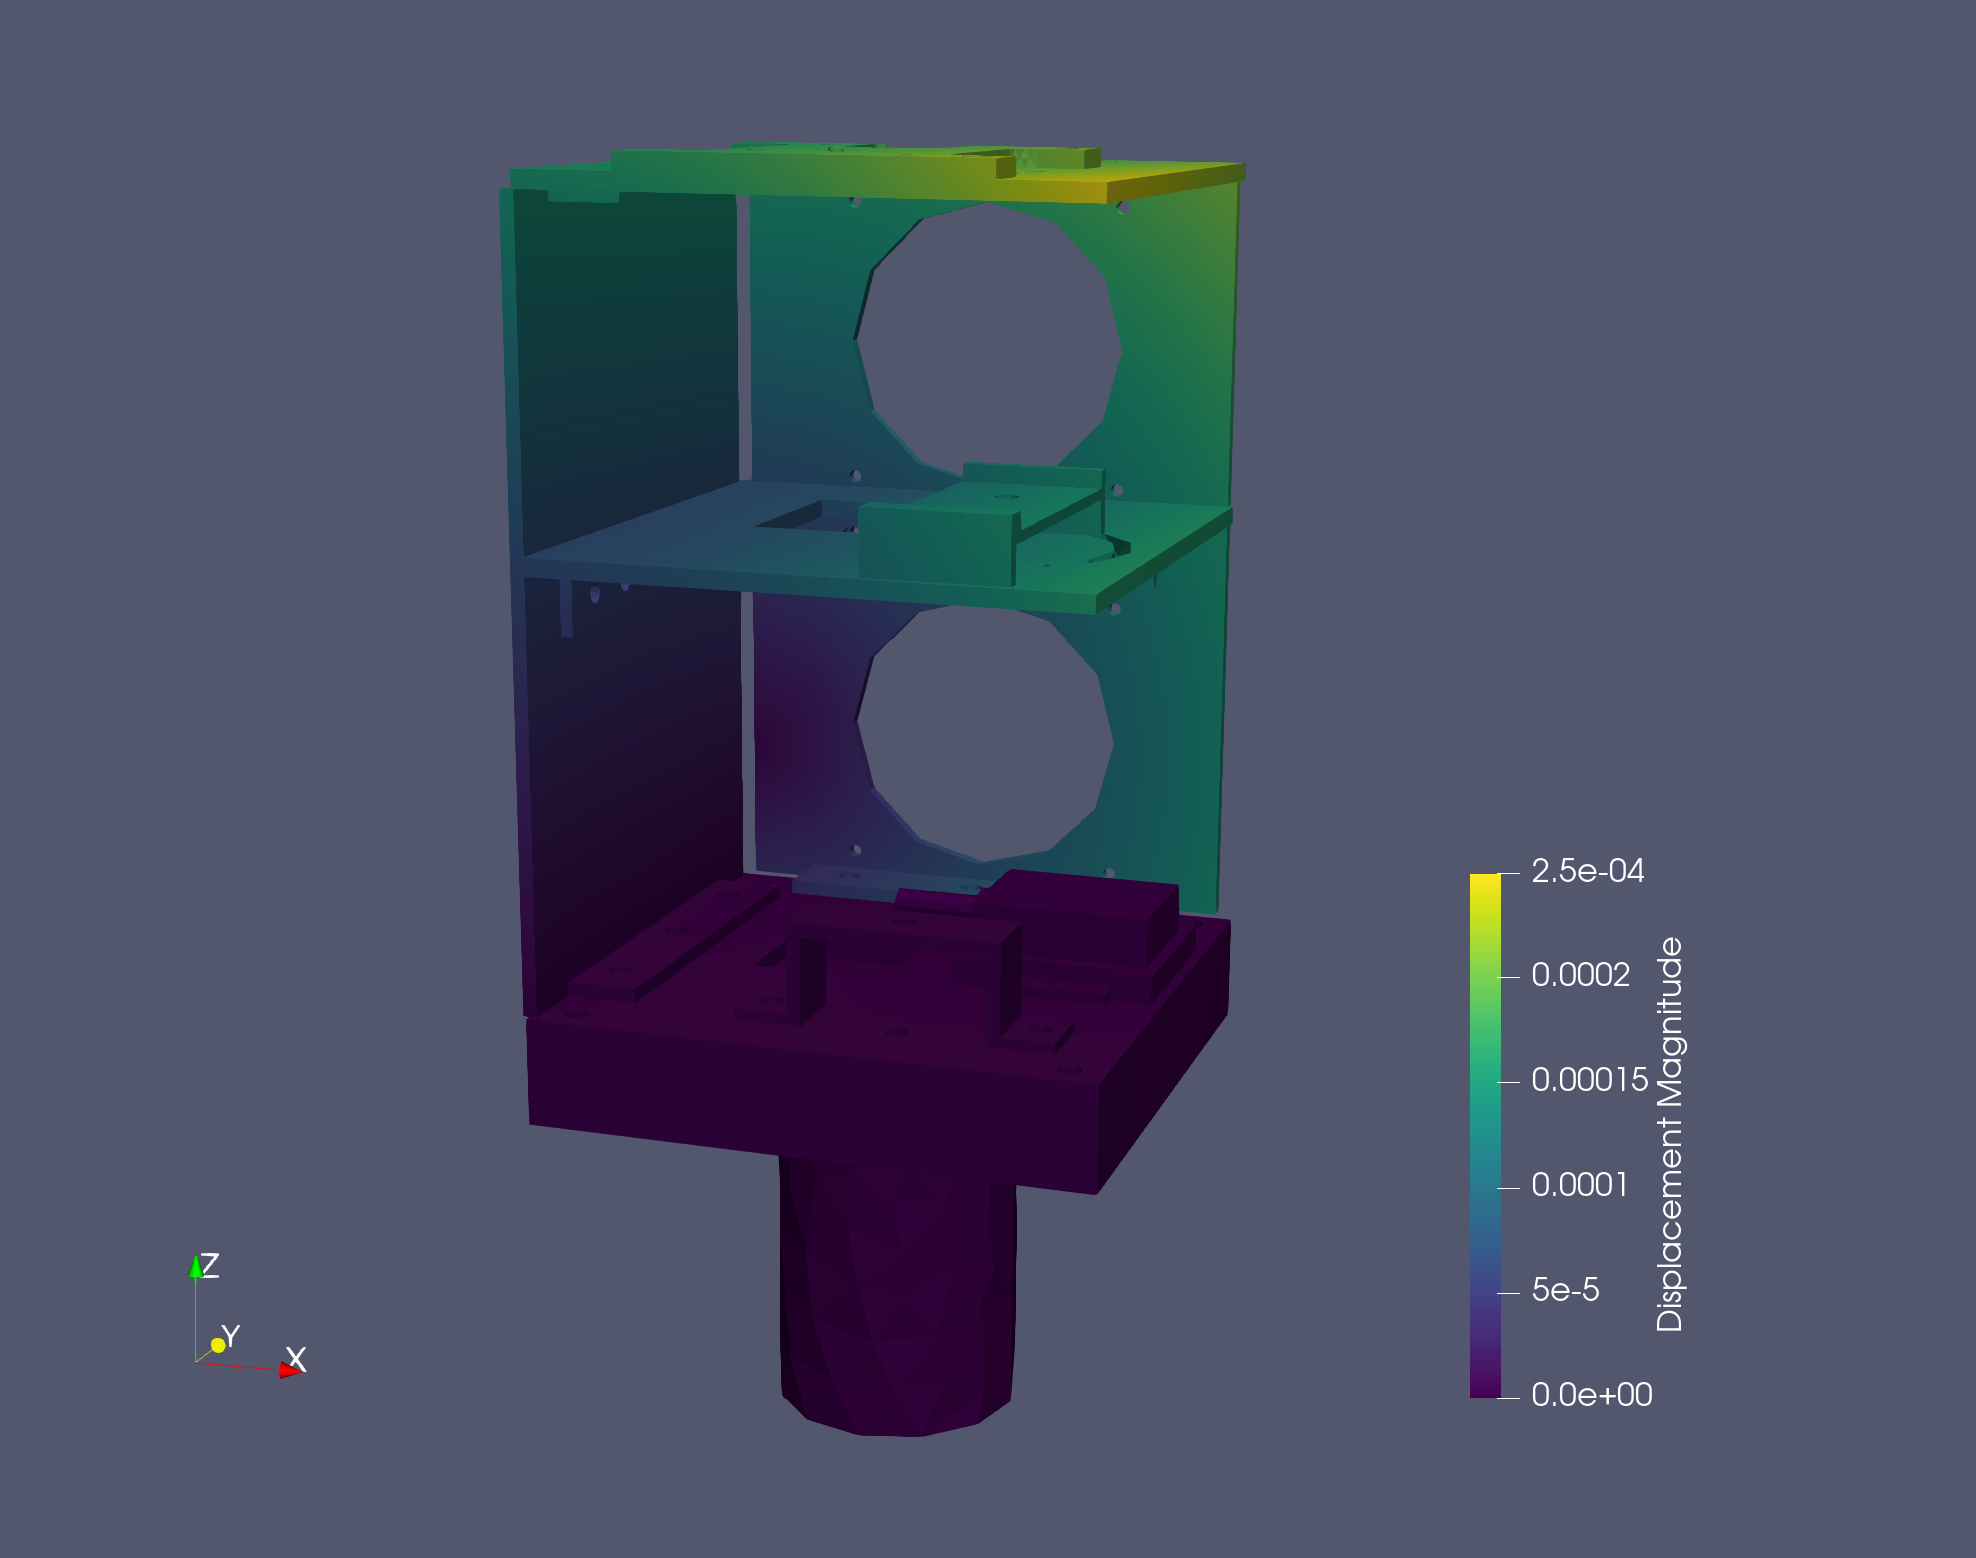
\includegraphics[width=0.9\linewidth]{images/stress_test1.png}
    \caption{Static tests stress in FreeCAD}
    \label{fig: static stress test}
\end{figure}

\todo[inline]{Talk about the collapsed bridge and importance of computing the natural frequencies}

While these tests might not be entiretly precise, knowing the natural frequency modes of the apparatus is two degrees of magnitude above the walking frequency is reassuring.




\section{Software Architecture}

\todo[inline]{Explain Docker infrastructure}

\todo[inline]{Add architecture of Android App (using the MMVC architecture)}